\chapter{PELAKSANAAN PENELITIAN}
\label{pelaksanaan-penelitian}

\section{Alat dan Bahan Penelitian}
Penelitian ini tidak dapat dilakukan tanpa adanya alat dan bahan yang memudahkan proses pelaksanaan penelitian. Alat dan bahan yang digunakan dijabarkan secara rinci pada Tabel \ref{tbl:4:alatbahan} dan Tabel \ref{tbl:4:speklaptop}.

\vspace{2em}
\begin{table}[!h]
	\caption{Daftar alat dan bahan}
	\label{tbl:4:alatbahan}
	\centering
	% use packages: array
	\begin{tabular}{|c|p{3.6cm}|p{9cm}|}
		\hline
		No. & Nama alat/bahan & Fungsi \\
		\hline
		1 & ASUS N550JX & Perangkat komputer \\ \hline
		2 & \textit{Climate chamber} & Objek penelitian \\ \hline
		3 & IES-VE 2019 & Perangkat lunak untuk pengambilan data lingkungan termal \textit{climate chamber} dan variasi gangguan \\ \hline
		4 & MS Excel 365 & Perangkat lunak pengolahan data tabular \\ \hline
		5 & MATLAB R2018a & Perangkat lunak pemrograman dalam merancang jaringan saraf tiruan untuk kontroler. \\ \hline
		6 & SIMULINK & Perangkat lunak untuk mewujudkan simulasi sistem kontrol. \\ \hline
		%5 & VS Code 1.38 & Aplikasi penulisan dan penyuntingan kode sumber \\ \hline
		%6 & Python 3.7 & Bahasa pemrograman \\ \hline
		%7 & Anaconda 3 & Distribusi pengelola lingkungan pengembangan dan manajemen paket untuk komputasi ilmiah \\ \hline
		%8 & Jupyter Notebook 1.0 & Aplikasi web untuk menulis kode program, teks, persamaan, dan visualisasi \\ \hline
		%9 & Pandas 1.0.3 & Pustaka manupulasi dan analisis data \\ \hline
		%10 & Scikit-Learn 0.21 & Pustaka pembangunan \textit{Machine Learning} \\ \hline
		%11 & fireTS 0.0.7 & Pustaka prediksi deret waktu multivarian \\ \hline
		%6 & Raspberry Pi versi 3 B & Komputer mikro sebagai perangkat pengendali. \\ \hline
	\end{tabular}
\end{table}

\begin{table}[!h]
	\caption{Spesifikasi laptop ASUS N550JX}
	\label{tbl:4:speklaptop}
	\centering
	% use packages: array
	\begin{tabular}{|c|p{5cm}|p{8cm}|}
		\hline
		No. & Komponen & Spesifikasi \\ \hline
		1 & \textit{Processor} & Intel Core i7-4720HQ CPU @ 2.60GHz x 8 \\ \hline
		2 & \textit{Graphics} & Intel Haswell Mobile \\ \hline
		3 & RAM & 8 GB \\ \hline
		4 & Tipe sistem operasi & 64-bit \\ \hline
		5 & Sistem operasi & Windows 10 Home Single Language \\ \hline
		%6 & Sistem operasi & Manjaro Linux \\ \hline
	\end{tabular}
\end{table}

\textit{Climate chamber} memiliki fungsi sebagai prasarana uji eksperimental pada penelitian yang menggunakan variabel lingkungan termal. Salah satu penelitian yang menggunakan \textit{climate chamber} yaitu penelitian mengenai kenyamanan termal.

\vspace{2em}
\section{Tata Laksana Penelitian}
Alur penelitian yang digunakan dalam mencapai tujuan dapat dilihat pada Gambar \ref{fig:4:TataLaksanaPenelitian} berikut.
\begin{figure}[!h]
	\centering
	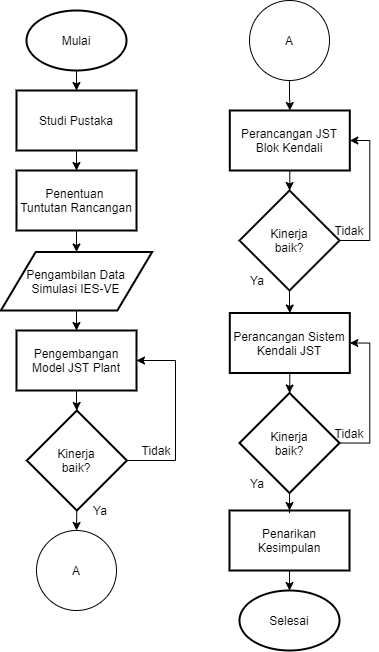
\includegraphics[width=0.6\textwidth]{figures/TataLaksanaPenelitian}
	\caption{Bagan Tata Laksana Penelitian}
	\label{fig:4:TataLaksanaPenelitian}
\end{figure}

%\begin{figure}[!h]
%	\centering
%	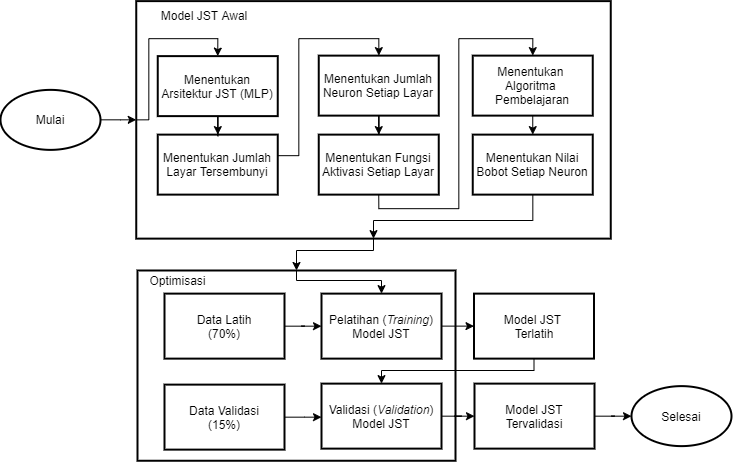
\includegraphics[width=0.85\textwidth]{figures/PerancanganModel}
%	\caption{Bagan Perancangan Model JST}
%	\label{fig:4:DiagramPerancanganModel}
%\end{figure}

%\begin{landscape}
%	\begin{figure}[!h]
%		\centering
%		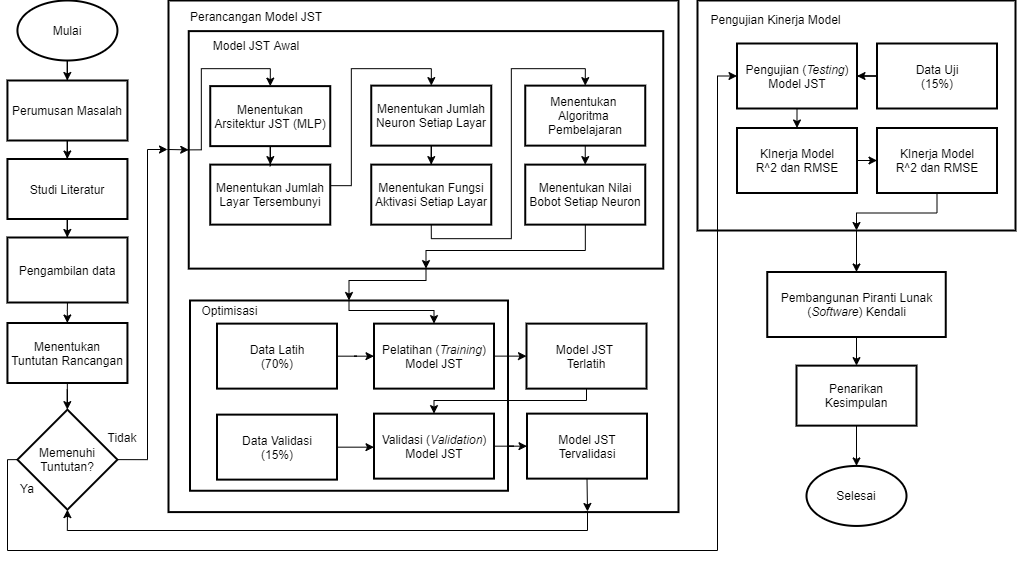
\includegraphics[width=1.5\textwidth]{figures/DiagramPenelitianFull}
%		\caption{Diagram Alir Penelitian Utuh}
%		\label{fig:4:DiagramPenelitianFull}
%	\end{figure}
%\end{landscape}

\subsection{Studi Pustaka}
Studi pustaka bertujuan untuk mendapatkan pemahaman dalam penyelesaian masalah yang diangkat dalam penelitian ini. Studi pustaka juga membantu menegaskan tujuan penelitian sehingga penulis mampu mengetahui perbedaan penelitian ini dengan penelitian terkait yang telah dilakukan sebelumnya. Dari studi pustaka yang telah dilakukan maka akan memperjelas tuntutan perancangan dari sistem yang akan dibuat. Informasi yang digunakan bersumber dari berbagai artikel ilmiah, jurnal, skripsi, buku, dan/atau sumber tertulis lainnya yang membahas mrengenai sistem kontrol lingkungan termal dan/atau jaringan saraf tiruan.

\subsection{Penentuan Tuntutan Rancangan}

Tuntutan rancangan Tugas Akhir ini yaitu kontroler mampu mengendalikan \textit{plant} pada skenario penggunaan \textit{climate chamber} dengan galat suhu kurang dari $\pm$1$^\circ$C dan galat kelembapan relatif kurang dari $\pm$10\%.


\subsection{Pengambilan Data Simulasi IES-VE}

Pada penelitian ini, digunakan model IES-VE untuk melakukan proses simulasi lingkungan termal. Bersamaan dengan penelitian Hartanto \cite{skripsiTanto}, data bersumber dari model yang telah dibuat pada penelitian sebelumnya berjudul "Karakterisasi Lingkungan Termal Chamber Iklim Menggunakan Metode Simulasi CFD dengan Perangkat Lunak IES-VE" yang diteliti oleh Kurniawan \cite{skripsiIchfan}.  Data tersebut merupakan hasil simulasi pada \textit{software} IES-VE dengan menerapkan beberapa variasi kondisi lingkungan pada model \textit{climate chamber}. Variasi tersebut yaitu kondisi batas lingkungan (radiasi matahari dan suhu bola kering luar/\textit{outdoor dry bulb temperature}), kondisi AC, dan kondisi \textit{heater}. Variasi kondisi batas lingkungan tersebut diwujudkan dalam pembagian 4 musim dalam 1 tahun, yakni bulan Maret, Juni, September dan Desember. Keluaran dari model IES-VE berupa nilai suhu ruang (\textit{air temperature}) \textit{chamber} dan kelembapan relatif (RH) \textit{chamber}. Dari model tersebut didapatkan nilai MAE perhitungan selisih variabel lingkungan termal hasil simulasi dan pengukuran lapangan sebesar 0,8 $\pm$ 0,7$^{\circ}$C untuk suhu udara ruang dan 2,5 $\pm$ 3,8\% untuk kelembaban relatif \cite{skripsiIchfan}. Data yang sudah terkumpul disajikan dalam bentuk tabular dan diolah dengan menggunakan komputer.\\

\noindent\textbf{Kondisi \textit{Climate Chamber}}

Climate chamber memiliki ukuran panjang $\times$ lebar $\times$ tinggi = 3 m $\times$ 2 m $\times$ 3 m. Komponen-komponen di dalam \textit{climate chamber} terdiri dari meja, kursi, \textit{blower}, penghuni, lampu, \textit{heater}, dan AC. Posisi setiap komponen di dalam \textit{climate chamber} digambarakan pada Gambar \ref{fig:4:KondisiChamber}.

\begin{figure}[!h]
	\centering
	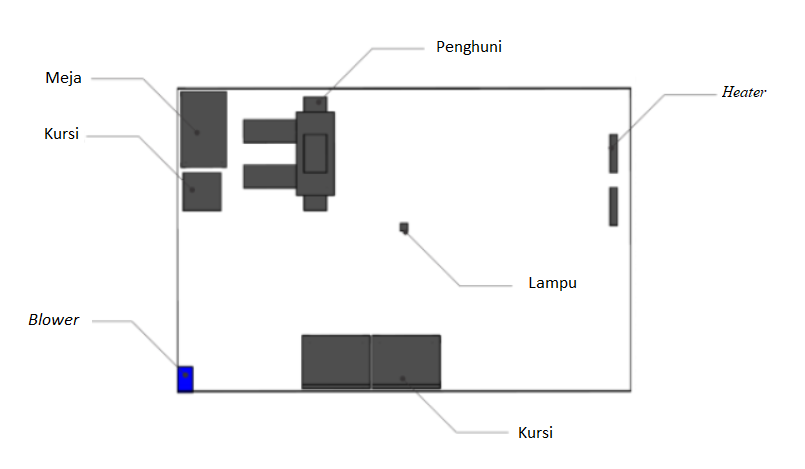
\includegraphics[width=1\textwidth]{figures/KondisiChamber}
	\caption{Posisi Komponen-Komponen di dalam \textit{Climate Chamber}}
	\label{fig:4:KondisiChamber}
\end{figure}
\vspace{3em}

Perangkat AC yang berada di dalam \textit{climate chamber} DTNTF FT-UGM memiliki daya sebesar 2800W (1 PK). Perangkat AC mampu mengkondisikan lingkungan melalui aliran udara yang keluar. Oleh karena itu, Perangkat AC sangatlah berpengaruh terhadap kondisi lingkungan termal di dalam ruangan. Penampakan wujud perangkat AC dapat dilihat pada Gambar \ref{fig:4:AC}

\begin{figure}[!h]
	\centering
	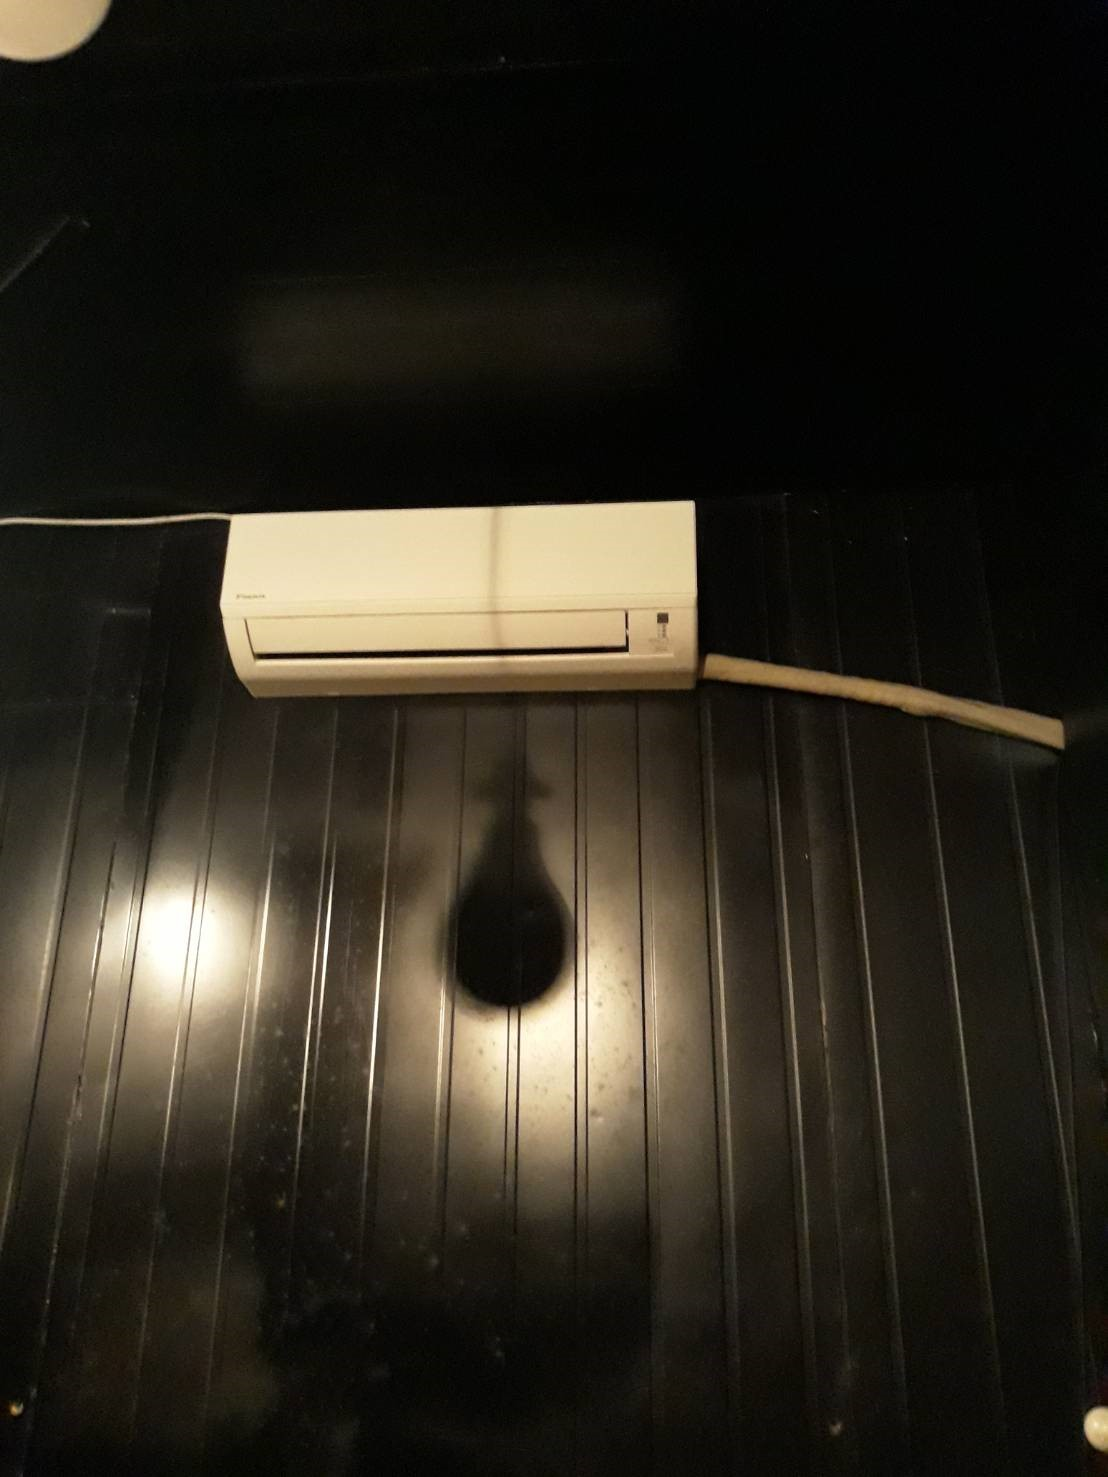
\includegraphics[width=0.35\textwidth]{figures/AC}
	\caption{Perangkat AC}
	\label{fig:4:AC}
\end{figure}

Perangkat pemanas (\textit{heater}) yang berada di dalam \textit{climate chamber} memiliki daya sebesar 900W. Terdapat dua buah perangkat pemanas di dalam \textit{climate chamber}. Semakin banyak perangkat pemanas yang aktif maka suhu ruang akan menjadi semakin meningkat. Kenaikan rerata suhu ruang yaitu sebesar $\pm1,9^\circ$C untuk setiap perangkat pemanas. Penampakan wujud \textit{heater} dapat dilihat pada Gambar \ref{fig:4:Heater}.

\begin{figure}[!h]
	\centering
	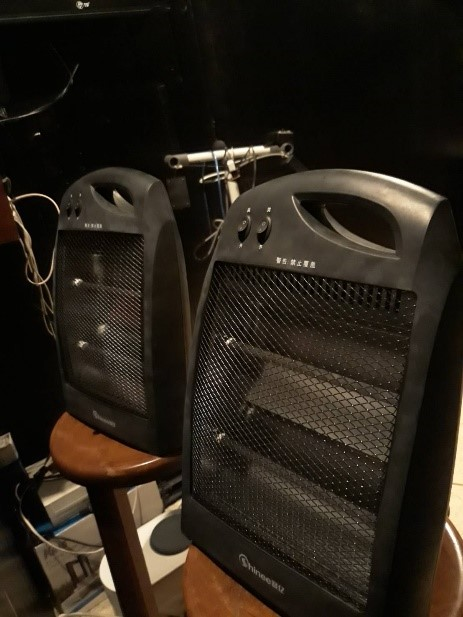
\includegraphics[width=0.2\textwidth]{figures/Heater}
	\caption{Perangkat Heater}
	\label{fig:4:Heater}
\end{figure}

Selain faktor di dalam \textit{climate chamber}, faktor dari luar ruangan pun secara tidak langsung mempengaruhi kondisi lingkungan termal \textit{climate chamber}, di antaranya adalah suhu lingkungan (\textit{dry bulb temperature}) dan intensitas radiasi matahari. Posisi harian matahari mempengaruhi perubahan nilai suhu lingkungan dan intensitas radiasi matahari. Pada siang hari (posisi \textit{altitude} matahari ketika berada tepat di atas \textit{climate chamber}) memberikan paparan radiasi matahari yang mengenai selubung bangunan. Hal ini menyebabkan kenaikan suhu di dalam \textit{climate chamber}.\\

\noindent\textbf{Rancangan Skenario Pengambilan Data}

Rancangan skenario pada \textit{climate chamber} menghasilkan kombinasi antara perangkat AC dan jumlah \textit{heater} dalam kondisi ON. Perangkat AC dikondisikan untuk menyala dari pukul 08:00 sampai dengan pukul 17:00 WIB bervariasi dengan rentang nilai 16$^\circ$C - 30$^\circ$C dengan lompatan 1$^\circ$C. Jumlah \textit{heater} dalam kondisi ON terbagi menjadi 3 kondisi, yaitu keduanya tidak menyala (berkode 0), salah satu menyala (berkode 1), dan keduanya menyala (berkode 2). Kombinasi tersebut menghasilkan 25 variasi skenario. Untuk variasi suhu lingkungan dan intensitas radiasi matahari digunakan 4 titik ekstrim bumi terhadap matahari yaitu pada tanggal 21 Maret, 21 Juni, 23 September dan 22 Desember. Kemudian dilakukan simulasi pada setiap titik tersebut dengan kombinasi pada Gambar \ref{fig:4:SkenarioData}. Dengan demikian, total skenario yang dihasilkan dari kombinasi tersebut berjumlah 100 skenario.

\begin{figure}[!h]
	\centering
	
\includegraphics[width=0.65\textwidth]{figures/SkenarioData}
	\caption{Skenario Pengambilan Data}
	\label{fig:4:SkenarioData}
\end{figure}
\vspace{1em}
\break
\break

\subsection{Model \textit{Plant} JST}
Model \textit{plant} pada penelitian ini menggunakan model JST yang telah dibangun oleh Hartanto pada \cite{skripsiTanto}. Arsitektur Model Plant JST digambarkan pada Gambar \ref{fig:4:NNPlantModelDesign}. Model plant yang digunakan memiliki nilai MAE perhitungan antara target dan prediksi sebesar 0,59$^{\circ}$C untuk suhu ruang dan 5,44\% untuk kelembapan relatif. Akurasi JST sebesar 96,23\% untuk suhu ruang dan 68,90\% untuk kelembapan relatif. Keseluruhan nilai \textit{hyperparameter} model JST yang dirangkum pada Tabel \ref{tbl:5:NNPlantTanto}.

\begin{figure}[!h]
	\centering
	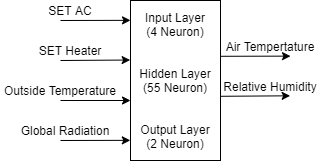
\includegraphics[width=0.65\textwidth]{figures/NNPlantModelDesign}
	\caption{Arsitektur Model Plant JST}
	\label{fig:4:NNPlantModelDesign}
\end{figure}

\begin{table}[!h]
	\caption{Tabel Rancangan Model Plant JST}
	\label{tbl:5:NNPlantTanto}
	\centering
	% use packages: array
	\begin{tabular}{|p{5cm}|p{5.2cm}|}
		\hline
		\textbf{Nama Hyperparameter} & \textbf{Nilai Hyperparameter} \\ \hline
		Arsitektur & Feedforward Neural Network \\ \hline
		Pembagian Data & 50\% 25\% 25\% \\ \hline 
		Jumlah Layar Tersembunyi & 1 \\ \hline
		Jumlah Neuron pada Layar & [55] \\ \hline
		Fungsi Aktivasi Layar & Hyperbolic Tangent \\ \hline
		Algoritma Pembelajaran & Levenberg-Marquardt \\ \hline
		Mean Absolute Error (MAE) & T$_{db}$: 0,59$^\circ$C ; RH: 5,44\% \\ \hline
		Mean Squared Error (MSE) & T$_{db}$: 0,75$^\circ$C ; RH: 52,33\% \\ \hline
		Koefisien Korelasi (R) & T$_{db}$: 96,23\% ; RH: 68,90\% \\ \hline
	\end{tabular}
\end{table}


\subsection{Perancangan Kontrol berbasis JST}

Dalam melakukan pemodelan kontrol, pertama-tama didefinisikan terlebih dahulu pasangan data masukan dan keluaran dari sistem kendali. Pasangan data masukan dan keluaran tersebut didapatkan dengan memperhatikan diagram blok sistem pengendalian yang ditunjukkan pada Gambar \ref{fig:4:ConstrolSystemBlockDiagram}. Nilai pasangan masukan dan keluaran kontrol ditunjukkan pada Gambar \ref{fig:4:NNControlIO}.

\begin{figure}[!h]
	\centering
	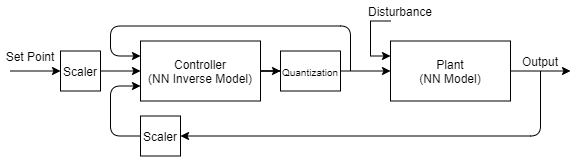
\includegraphics[width=1\textwidth]{figures/ControlDesignDiagramII}
	\caption{Diagram blok sistem kontrol berbasis JST \cite{paper42Paisan}}
	\label{fig:4:ConstrolSystemBlockDiagram}
\end{figure}

\begin{figure}[!h]
	\centering
	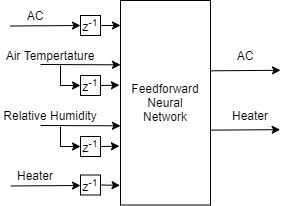
\includegraphics[width=0.5\textwidth]{figures/NNControllerIO}
	\caption{Pasangan masukan dan keluaran model JST kontroler}
	\label{fig:4:NNControlIO}
\end{figure}

Kontroler dibangun dari model JST dengan menggunakan prinsip model invers dari model \textit{plant}. Perancangan JST untuk kontroler menggunakan \textit{delay} umpan balik AC, \textit{delay} umpan balik \textit{heater}, output \textit{plant} dan \textit{delay} output \textit{plant} sebagai sebagai masukan untuk pelatihan JST. Kemudian, pasangan data AC dan \textit{heater} digunakan sebagai pasangan data keluaran (data target) untuk pelatihan JST. Arsitektur JST kontroler dibangun dengan menggunakan \textit{feedforward neural network} atau biasa disebut juga sebagai \textit{multilayer perceptron} (MLP). Model JST akan dilatih menggunakan data hasil simulai IES-VE yang telah digunakan pula dalam pemodelan \textit{plant} oleh Hartanto \cite{skripsiTanto}. Pada proses pelatihan JST, dilakukan penskalaan terhadap semua input JST menggunakan metode \textit{Min Max Scaling} kecuali variabel \textit{delay} umpan masuk AC dan \textit{heater}. Penskalaan bertujuan untuk meningkatkan kinerja JST menjadi optimal dengan menyamakan rentang nilai dan besar satuan dari setiap variabel (berupa rentang nilai dari 0 hingga 1).

Perancangan model JST kontroler dilakukan dengan membandingkan variasi pembagian data latih, data validasi, dan data uji. Kemudian akan divariasikan pula fungsi aktivasi dan jumlah neuron untuk memperoleh model JST yang optimal. Evaluasi kinerja model JST kontroler menggunakan perbandingan nilai MSE pada setiap rancangan. Rancangan model JST dengan nilai MSE terkecil akan digunakan sebagai model kontroler.

\subsection{Penarikan Kesimpulan}
Penarikan kesimpulan didapatkan berdasarkan hasil rancangan kontroler dengan kinerja dari model jaringan saraf tiruan di dalamnya. Kesimpulan menggambarkan bagaimana rancangan kontroler dapat digunakan pada \textit{climate chamber}.

\section{Rencana Analisis Hasil Penelitian}
Kinerja model JST akan dievaluasi berdasarkan nilai MAE (\textit{Mean Absolute Error}) dan R (koefisien korelasi) dari rancangan tersebut. Kinerja dari kontroler akan dievaluasi berdasarkan nilai rerata galat (\textit{steady-state error}) untuk suhu ruang dan kelembapan relatif.